

\tikzset{every picture/.style={line width=0.75pt}} %set default line width to 0.75pt        

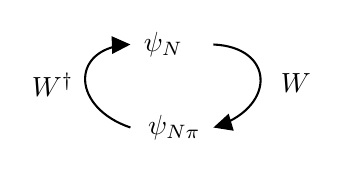
\begin{tikzpicture}[x=0.75pt,y=0.75pt,yscale=-1,xscale=1]
	%uncomment if require: \path (0,300); %set diagram left start at 0, and has height of 300
	
	%Curve Lines [id:da45911359937309637] 
	\draw    (280,60) .. controls (309.18,61.28) and (310.43,89.17) .. (282.66,99.13) ;
	\draw [shift={(280,100)}, rotate = 343.41] [fill={rgb, 255:red, 0; green, 0; blue, 0 }  ][line width=0.08]  [draw opacity=0] (8.93,-4.29) -- (0,0) -- (8.93,4.29) -- cycle    ;
	%Curve Lines [id:da6231994153364976] 
	\draw    (240,100) .. controls (211.9,90.47) and (210.92,62.94) .. (237.05,60.2) ;
	\draw [shift={(240,60)}, rotate = 178.19] [fill={rgb, 255:red, 0; green, 0; blue, 0 }  ][line width=0.08]  [draw opacity=0] (8.93,-4.29) -- (0,0) -- (8.93,4.29) -- cycle    ;
	
	% Text Node
	\draw (245,52.4) node [anchor=north west][inner sep=0.75pt]    {$\psi _{N}$};
	% Text Node
	\draw (247,92.4) node [anchor=north west][inner sep=0.75pt]    {$\psi _{N\pi }$};
	% Text Node
	\draw (191,72.4) node [anchor=north west][inner sep=0.75pt]    {$W^{\dagger }$};
	% Text Node
	\draw (311,72.4) node [anchor=north west][inner sep=0.75pt]    {$W$};
	
	
\end{tikzpicture}